\documentclass{article}
\usepackage{graphicx}
\usepackage{graphicx} 
\usepackage{amssymb}
\usepackage{float}
\usepackage{amsmath}
\usepackage{algorithm}
\usepackage{algpseudocode}
\usepackage{indentfirst}

\title{Polynomial Basis}
\author{ }
\date{ }

\begin{document}
	
	\maketitle 

    \section{Reducing Perceptron-Not-Through-Origin to Perceptron-Through-Origin}
    
    As promised earlier, the problem of perceptron-not-through-origin can be reduced to the problem of perceptron-through-origin. The key lies in transforming the dataset used from the $\mathbb{R}^d$ space to a $\mathbb{R}^D$ space when $D > d$. \\
    
    Recall that the parameters of a separator not through the origin are $\theta=[\theta_1, ... \theta_d]$ and $\theta_0$, a scalar. Say that these two parameters are taken to create a single one called $\theta_{new}$: $\theta_{new} = [\theta_1, ... \theta_d, \theta_0]$. $\theta_{new}$ is basically just $\theta$ with $\theta_0$ put in as the last entry. Now, each $x$ value vector in the dataset must also be modified. Say that $x_{new} = [x_1, ...,x_d,1]$. $x_{new}$ is basically just $x$ with $1$ put in as the last entry. $\theta^T_{new}x_{new} = \theta_1x_1 + ... + \theta_dx_d+(1)\theta_0=\theta_1x_1+...+\theta_dx_d+\theta_0=\theta^Tx+\theta_0$. A classifier-not-through-origin in $d$ dimensions can be turned into a classifier-through-origin in $d+1$ dimensions. Thus, even though the perceptron convergence theorem from before was only proved for perceptron through origin, transformation shows that the theorem also applies to perceptron-not-through-origin. \\

    \begin{figure}[H]
        \centering
        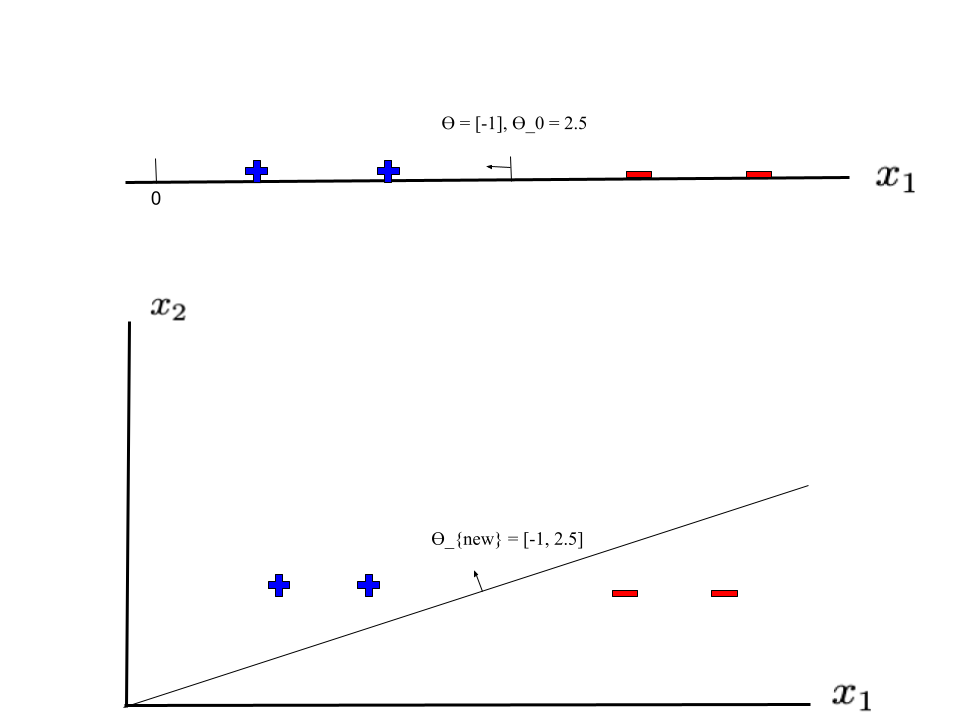
\includegraphics[width=0.5\linewidth]{Perceptron-Not-Through-Origin to Perceptron-Through-Origin.png}
    \end{figure}

    \section{Polynomial Basis}
    The same concept can be applied to a dataset that is not linearly separable in $d$ dimensions. By moving the dataset into $d+1$, $d+2$, or more generally, $d+n$ dimensions, one can make it linearly separable. 
    
    \begin{figure}[H]
        \centering
        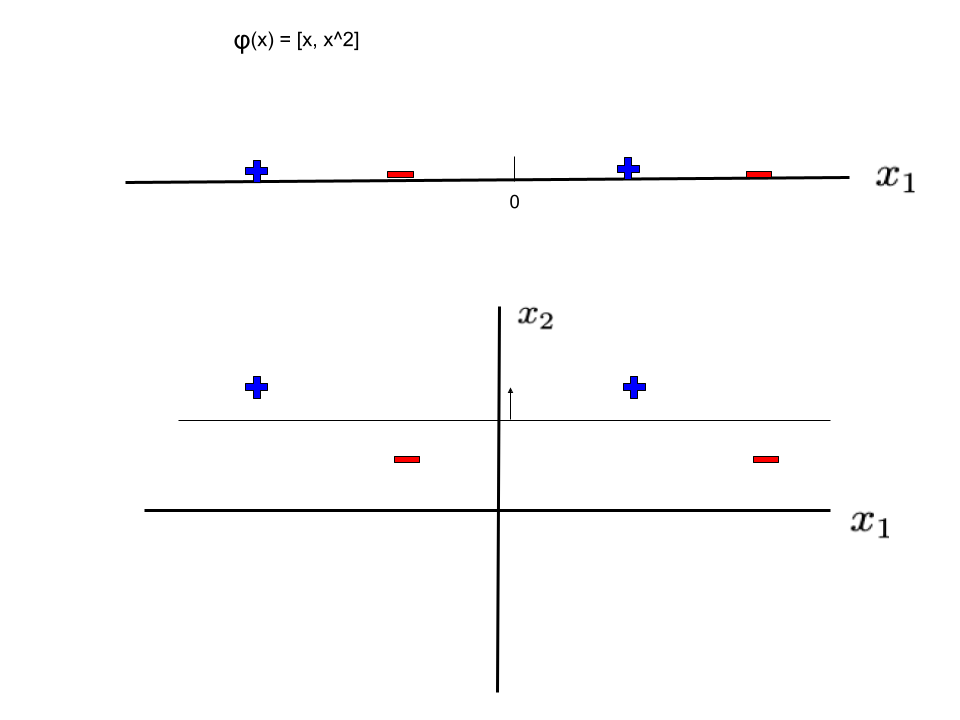
\includegraphics[width=0.5\linewidth]{Linearly Separable in Higher Dimensions.png}
    \end{figure}
    
    A systematic way of transforming data into higher dimensions exists. It is called polynomial basis. \\
    \begin{center}
        \begin{tabular}{ c c c }
         order & in general \\ 
         \hline
         0 & $[1]$ \\  
         1 & $[1, x_1, ... x_d]$ \\
         2 & $[1, x_1, ... x_d, x_1^2, x_1x_2, ... \text{all two way products}]$ \\
         3 & $[1, x_1, ... x_d, x_1^2, x_1x_2, ... \text{all two way products}, x_1^3, ... \text{all three way products}]$ \\
         ... & ... 
        \end{tabular}
    \end{center}

    For an example, take $[x_1, x_2]$. Using polynomial basis to transform it to the second degree yields $[1, x_1, x_2, x_1^2, x_1x_2, x^2]$.

    
    
\end{document}



























